\section{Linguaggi utilizzati}

\subsection{HTML5}
Il gruppo ha utilizzato il linguaggio di markup \textit{HTML5} per la modellazione delle pagine web.
Seguendo quanto imparato durante il corso di Tecnologie Web, l'attenzione si è focalizzata sulle
seguenti peculiarità:
\begin{itemize}
	\item \textit{Meta-tag}: nella sezione head dei documenti sono stati inseriti meta-tag necessari per
	migliorare l'accessibilità verso i motori di ricerca. Questo permette al sito di avere una buona
	visibilità nelle SERP;
	\item \textit{Separazione tra struttura, presentazione e comportamento}: il codice HTML non contiene
	codice CSS embedded, stili inline o codice di scripting (\textit{JS} o \textit{PHP}). Questi devono
	essere codificati in file separati e importati nella sezione head dei documenti \textit{HTML} che
	li richiedono.
\end{itemize}

\subsection{PHP}
Il lato server è stato sviluppato utilizzando il linguaggio di programmazione \textit{PHP}.\\
\\
É stata codificata una classe di supporto che funge da intermediaria tra gli script \textit{PHP} e le
chiamate al database, che si occupa di:
\begin{itemize}
	\item Gestire la connessione con il database;
	\item Fornire funzioni standard per recuperare dati dal database;
	\item Eseguire inserimenti, cancellazioni, modifiche.
\end{itemize}
Gli altri script verificano innanzitutto, se serve, se un utente è loggato. In seguito eseguono una
verifica dell'input ed aprono una connessione sul database interagendo con lo stesso. Al termine delle
operazioni, la connessione viene chiusa e se serve restituiscono a video i risultati con il comando
\texttt{echo}.\\
\\
Per assicurarsi che non ci siano tentativi di \textit{SQL injection}, sono stati implementati il controllo dell'input ed e stata utilizzata la funzione \texttt{mysqli{\_}real{\_}escape{\_}string} che si assicura che ogni carattere dell'input sia interpretato come testo.

\subsection{SQL}
SQL è stato utilizzato per la codifica del database, il quale è formato dalle seguenti tabelle:
\begin{itemize}
	\item \textit{Utente}: Contiene le informazioni di ogni utente;
	\item \textit{Bonus}: Contiene i bonus disponibili per ogni utente;
	\item \textit{Tavolo}: Contiene i tavoli presenti nel locale;
	\item \textit{Prenotazione}: Contiene le prenotazioni effettuate per ogni tavolo;
	\item \textit{Ordinazione}: Contiene le ordinazioni fatte da ogni utente;
	\item \textit{Acquisto}: Contiene le ordinazioni con i loro relativi elementi del listino selezionati;
	\item \textit{Elemento listino}: Contiene tutti gli elementi che sono disponibili alla vendita;
	\item \textit{Pizza}: Contiene tutte le pizze;
	\item \textit{Bevanda}: Contiene tutte le bevande;
	\item \textit{Dolce}: Contiene tutti i dolci;
	\item \textit{Ingrediente}: Contiene tutti gli ingredienti delle pizze;
	\item \textit{Composizione}: Contiene la relativa composizione di ingredienti di ogni pizza.
\end{itemize}
Le tabelle \textit{Utente, Prenotazione, Ordinazione e Acquisto} vengono riempite dinamicamente dagli
utenti tramite chiamate \textit{PHP}.\\
\\
Le tabelle \textit{Pizza, Bevanda, Dolce, Ingrediente e Composizioni} sono modificate dinamicamente da un
utente amministratore.
\begin{figure}[H]
	\centering
	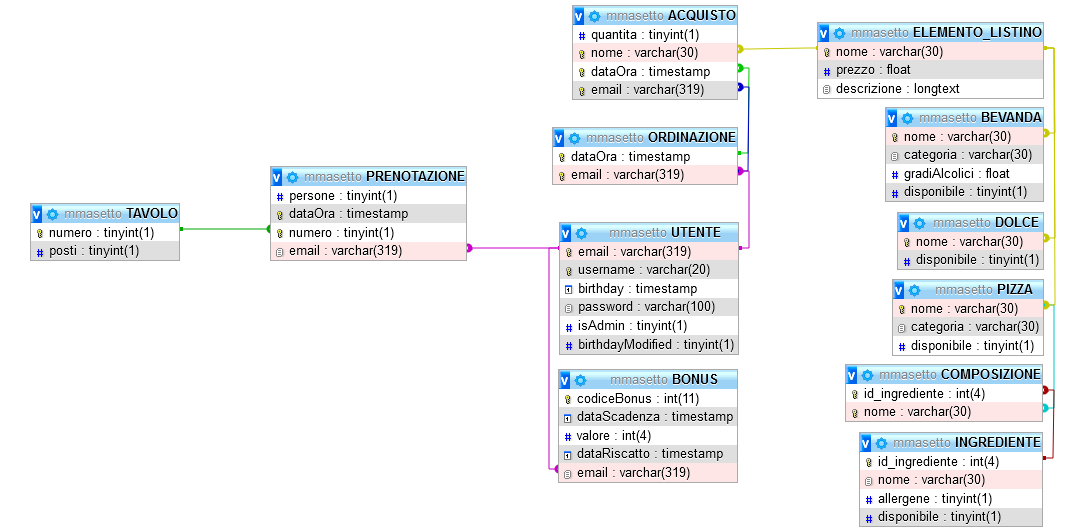
\includegraphics[scale=0.4]{resources/database_model.png}
	\caption{Modello del database}
\end{figure}

\newpage
\subsection{JavaScript}
\textit{JavaScript} è stato utilizzato per rendere il sito più dinamico e migliorare l'esperienza utente.
Occorre precisare però che la sua disabilitazione o il suo mancato funzionamento non comportano in alcun
modo l'impossibilità di fruire dei servizi offerti dal sito.\\
\\
In primo luogo, viene utilizzato al caricamento delle pagine del sito per verificare tramite una
chiamata \textit{AJAX} se c'è un utente loggato, e nel caso modificare il funzionamento del pulsante
\textit{"Accedi"} in modo tale che, oltre a mostrare la scritta \textit{"Il mio account"}, al suo click
mostri un menù a tendina con vari servizi che l'utente ha a sua disposizione. Se \textit{JavaScript} non
è presente, tali servizi saranno fruibili attraverso la navigazione del sito, e nel caso in cui non sia
stato fatto l'accesso l'utente verrà indirizzato alla pagina di login.\\
\\
Un altro suo scopo è quello di settare dinamicamente degli attributi \textit{ARIA} per migliorare
l'accessibilità del sito, in particolare per fornire maggiori informazioni allo screen reader e quindi
all'utente.\\
\\
Un suo altro utilizzo è quello di fornire la funzionalità mostra/nascondi password. Ovviamente la sua
mancanza non comporta alcun disagio all'utente.\\
\\
Infine viene utilizzato per effettuare chiamate \textit{AJAX} che restituiscono per l'utente loggato le
sue prenotazioni, i suoi acquisti e i suoi bonus, filtrati. Nel caso di non funzionamento di
\textit{Javascript}, non verrà effettuata alcuna chiamata \textit{AJAX}, ma semplicemente si mostreranno
tutti i dati dell'utente.